\chapter{Experimental work and results in mixed mode}
\label{Chapter2}

\section{Introduction}

In this section, the results obtained in mixed mode are presented. The decoupling of the modes has allowed to obtain the share of mode I and II. The imposed displacement compliance method has been used to calculate the different energy restitution rates. The deformation maps, force vs Crack Tip Opening curves, energy restitution rate vs crack length for different angles are presented below. It was decided to use only method 1 to measure the crack length as this method appears to be more accurate. The values of the GI - GII difference are also given. The calculation of the difference is intended to show the behaviour and evolution of the two modes with respect to the variation of the angle.

\section{Experimental set-up and method}

In mixed mode, this camera has the same inclination as the specimen, as shown in Figure \ref{fig:Setup15°}. The crack opening values are therefore projected directly along the x and y axes. The force is projected along the x and y axes, as shown in Figure \ref{fig:fig37bis}.

\begin{figure}[htp]
	\centering
	\includegraphics[width=16cm]{Setup15°}
	\caption{Experimental set-up}
	\label{fig:Setup15°}
\end{figure}

\section{Results}

\subsection{Deformation maps}

Figure \ref{fig:Strain_def_mixedmode} shows the deformation maps for the two tilt angles of the specimen in mixed mode which are 15° and 30°. Indeed, we did not have enough specimens to obtain results with 45°. These maps are given in terms of x (pixels) and y (pixels) coordinates. On these different deformation maps, we can clearly see the progression of the crack. The crack propagation path, although not perfectly straight, does not appear to change direction. As in Chapter 3, cracks tend to propagate according to the orientation and inclination of the fibres.

\begin{figure}[htp]
	\centering
	\begin{tabular}{c}
		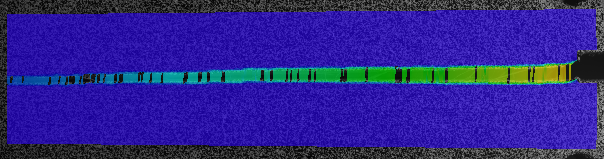
\includegraphics[width=8cm]{e15e2} \\
		e15e2 deformation map \\
		\\
		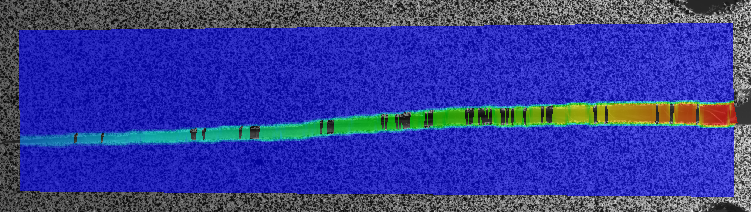
\includegraphics[width=8cm]{e30e3} \\
		e30e3 deformation map \\
		\\
		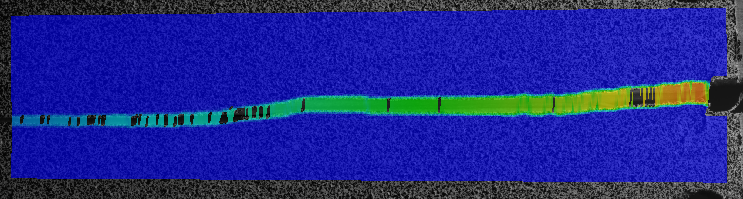
\includegraphics[width=8cm]{e30e5} \\
		e30e5 deformation map \\
	\end{tabular}
	\caption{Typical deformation map ($\epsilon$yy) obtained with DIC for mixed mode}
	\label{fig:Strain_def_mixedmode}
\end{figure}

As in the previous chapter, some curves are verified using deformation maps. Indeed, it is possible to read the crack tip graphically  on the deformation maps. Figure \ref{fig:e15e1_graphicread} and \ref{fig:e30e2_graphicread} show e15e1 and e30e2 verified by graphic reading. It seems that the crack length has been correctly estimated for each stage with method 1.

\begin{figure}[htp]
	\begin{minipage}[c]{.46\linewidth}
		\centering
		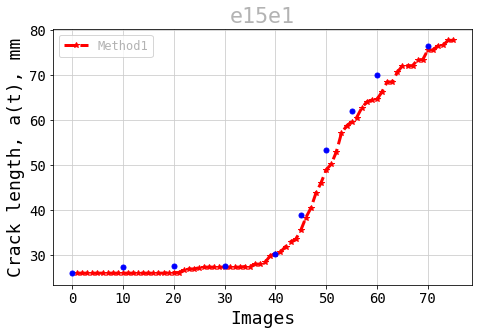
\includegraphics[width=8cm]{e15e1_graphicread}
		\caption{Crack tip by graphic reading e15e1}
		\label{fig:e15e1_graphicread}
	\end{minipage}
	\hfill%
	\begin{minipage}[c]{.46\linewidth}
		\centering
		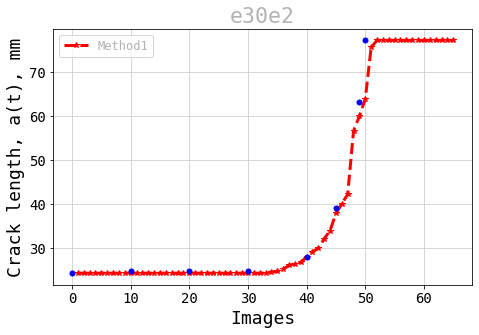
\includegraphics[width=8cm]{e30e2_graphicread}
		\caption{Crack tip by graphic reading e30e2 }
		\label{fig:e30e2_graphicread}
	\end{minipage}
\end{figure}

\subsection{Force - Crack Tip Opening Curve}

Figure \ref{fig:CTOD15} shows the evolution of the force as a function of the crack tip opening for 15°. For all the specimens, when a sudden drop in P is observed, signifying the complete failure of the material, the values along the x axis are less than 0.15 mm and of the order of 0.5 to 1.1 mm along the y axis.

\begin{figure}[H]
	\centering
	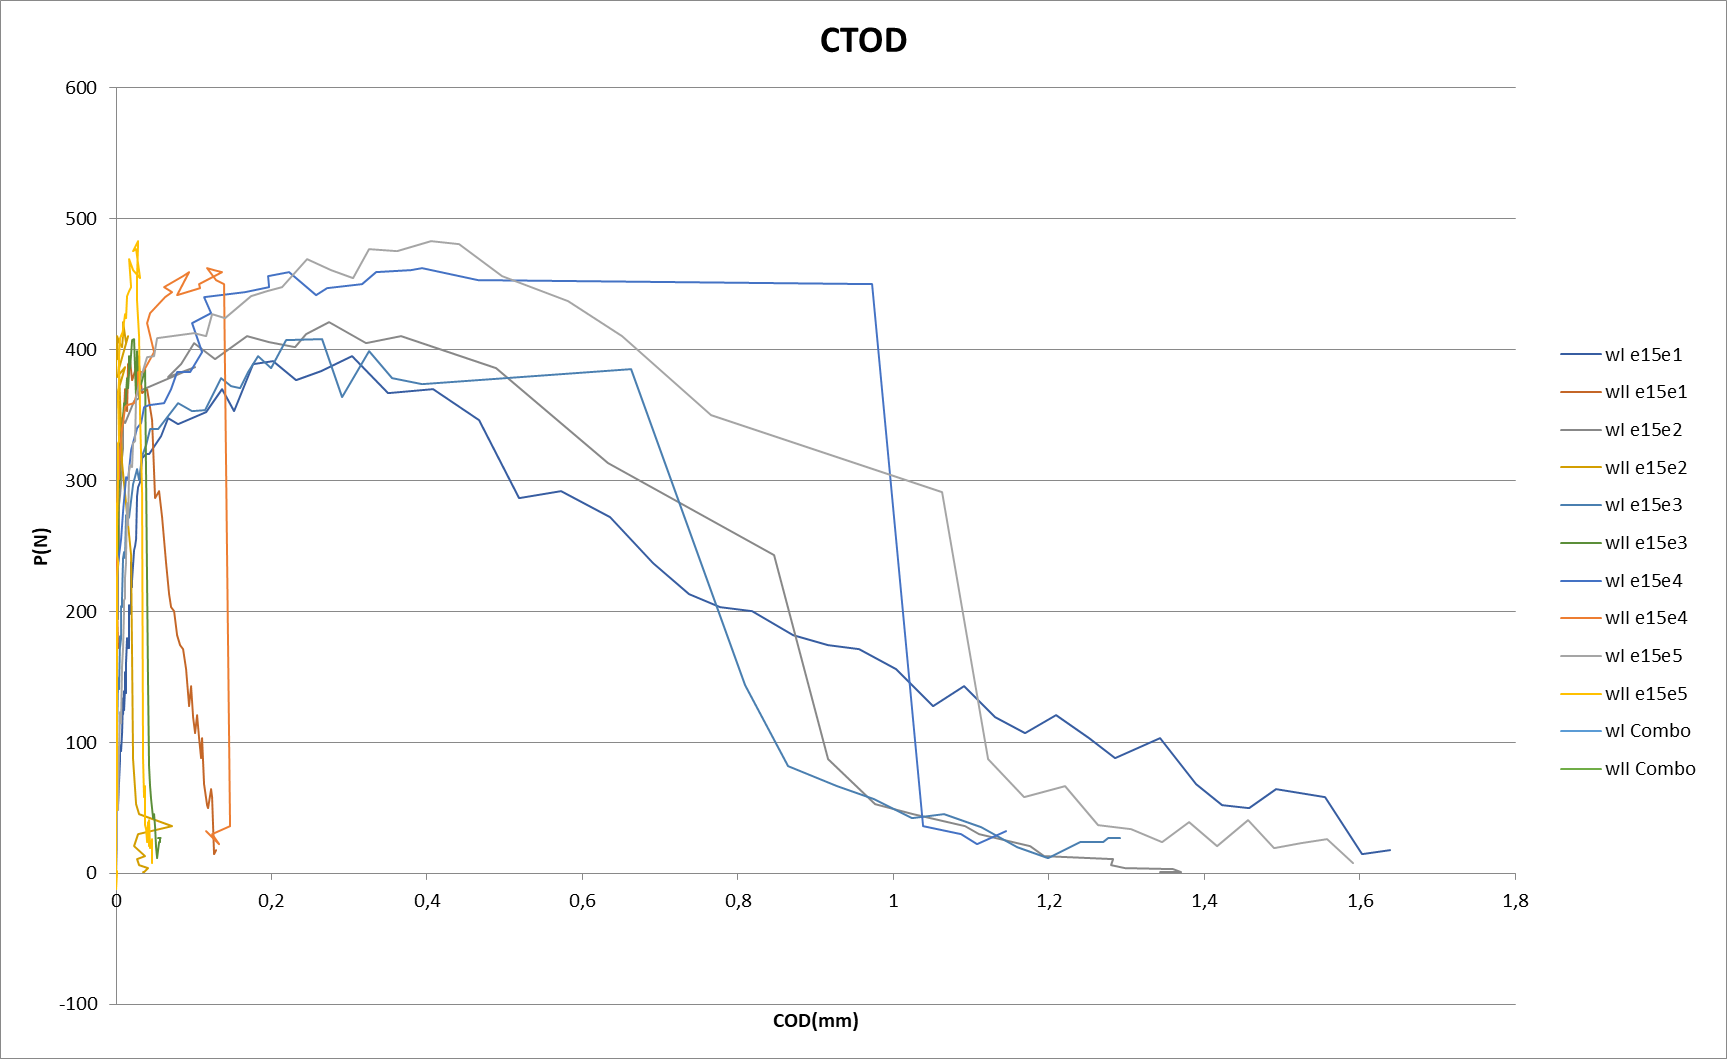
\includegraphics[width=15cm]{CTOD15}
	\caption{Evolution of the force as a function of the crack opening for 15° inclination}
	\label{fig:CTOD15}
\end{figure}

Figure \ref{fig:CTOD30} shows the force curves as a function of the crack opening for 30°. As can be seen, the crack opening along x for all the specimens tested is less than 0.11 mm. For the crack opening along y when a sudden drop in P is observed, the values are of the order of 0.4 to 1.1 mm. 
We can also see that the CTOD of e30e2 does not have the expected shape. After the image 53 of 66, the CTOD is not recorded correctly. However, this is of no real importance as P decreases sharply at stage 49, so it has no impact on the calculation of Gmax.

\begin{figure}[H]
	\centering
	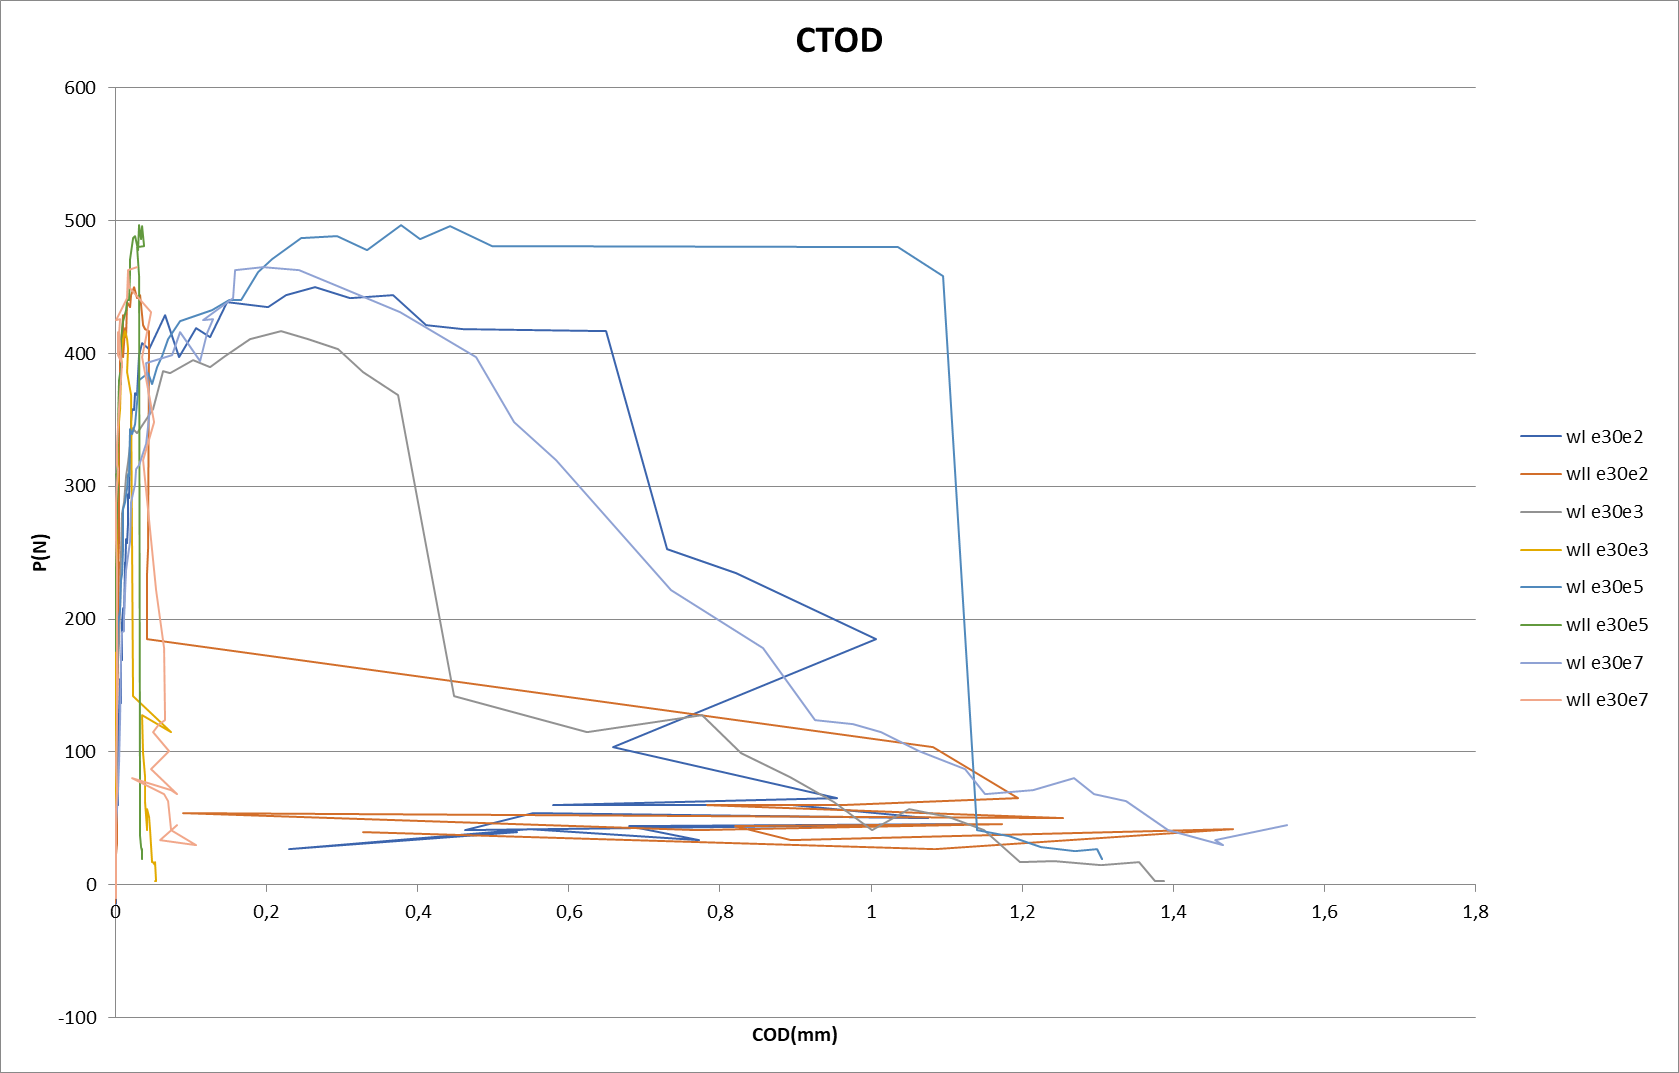
\includegraphics[width=15cm]{CTOD30}
	\caption{Evolution of the force as a function of the crack opening for 30° inclination}
	\label{fig:CTOD30}
\end{figure}

We can say that for 15° and 30° the crack openings along the x-axis are negligible compared to those along the y-axis. 

\subsection{Crack length curves}

All the crack length curve in function of displacement in mixed mode are shown in figure \ref{fig:crack_15} and \ref{fig:crack_30}. 
There are, as expected, different plateaus for the crack length. The crack length increases gradually and continuously before rupture. It is interesting to examine all the crack length propagation plots.  The curves are all more or less the same shape, and the crack ends at roughly the same length. What differs is the stage at which the crack begins to propagate. There are no major differences in crack length when you switch from mode I to mixed mode.

\begin{figure}[htp]
	\centering
	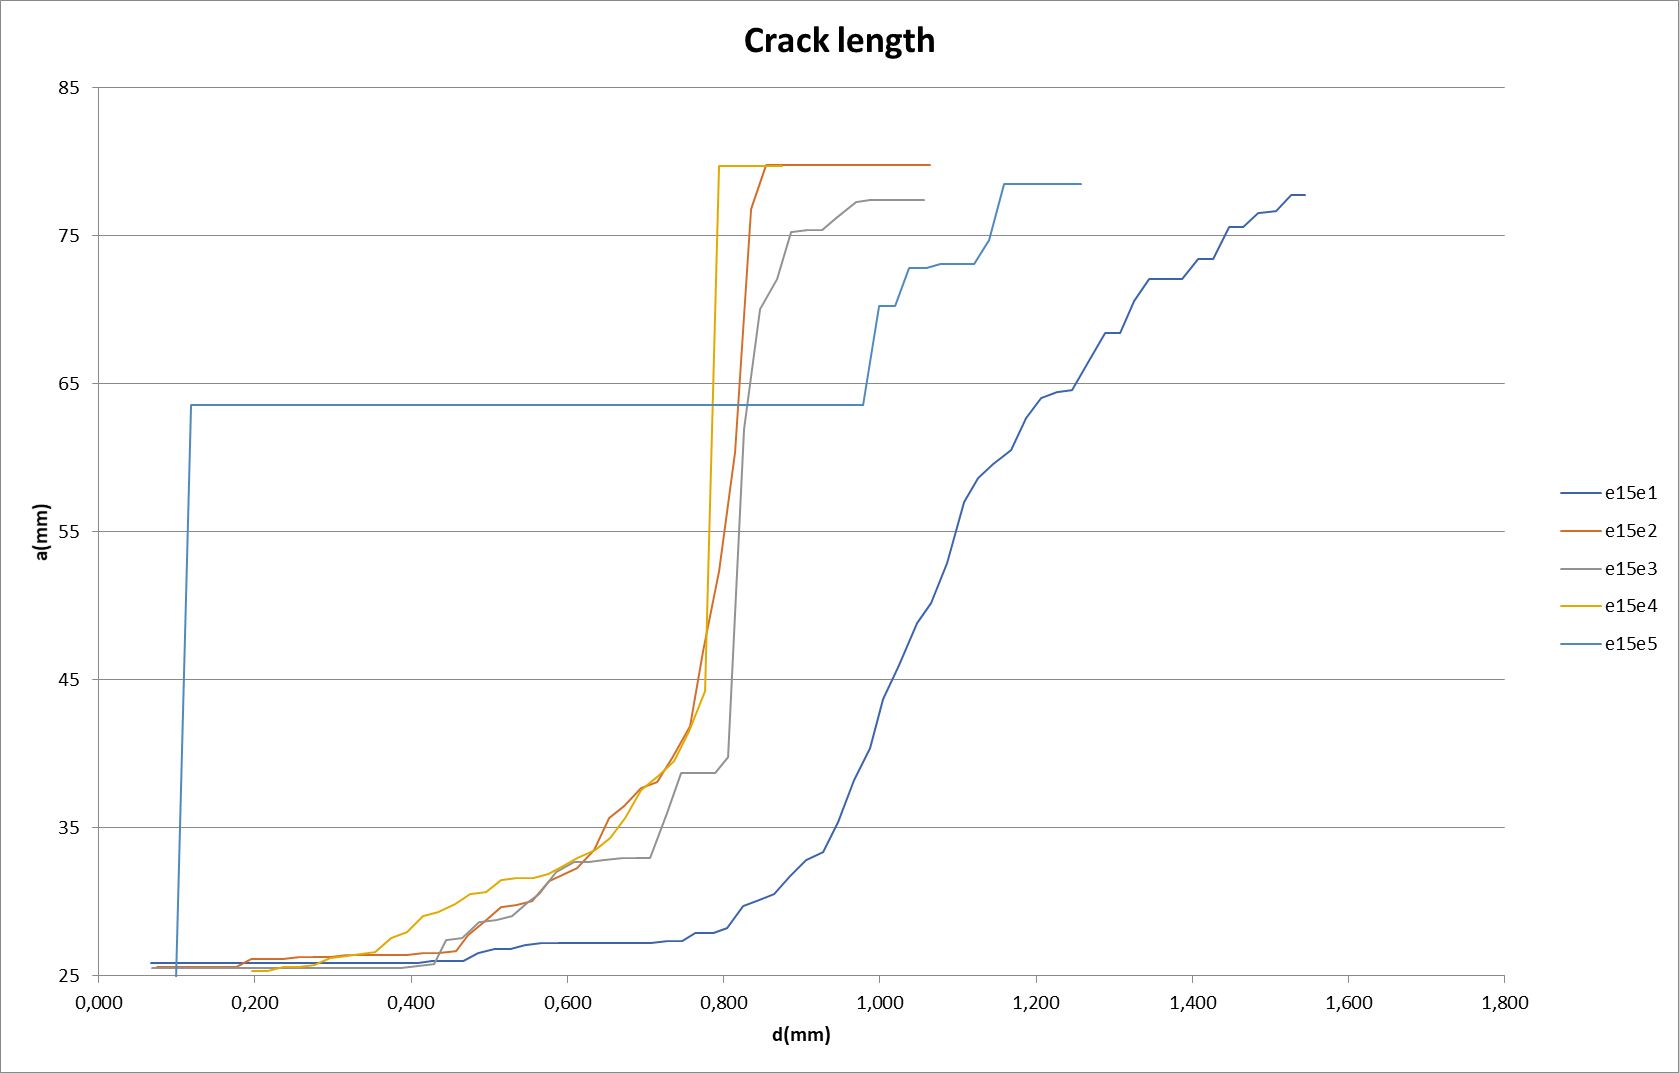
\includegraphics[width=13cm]{crack_15}
	\caption{Crack length evolution for 15°}
	\label{fig:crack_15}
\end{figure}

\begin{figure}[htp]
	\centering
	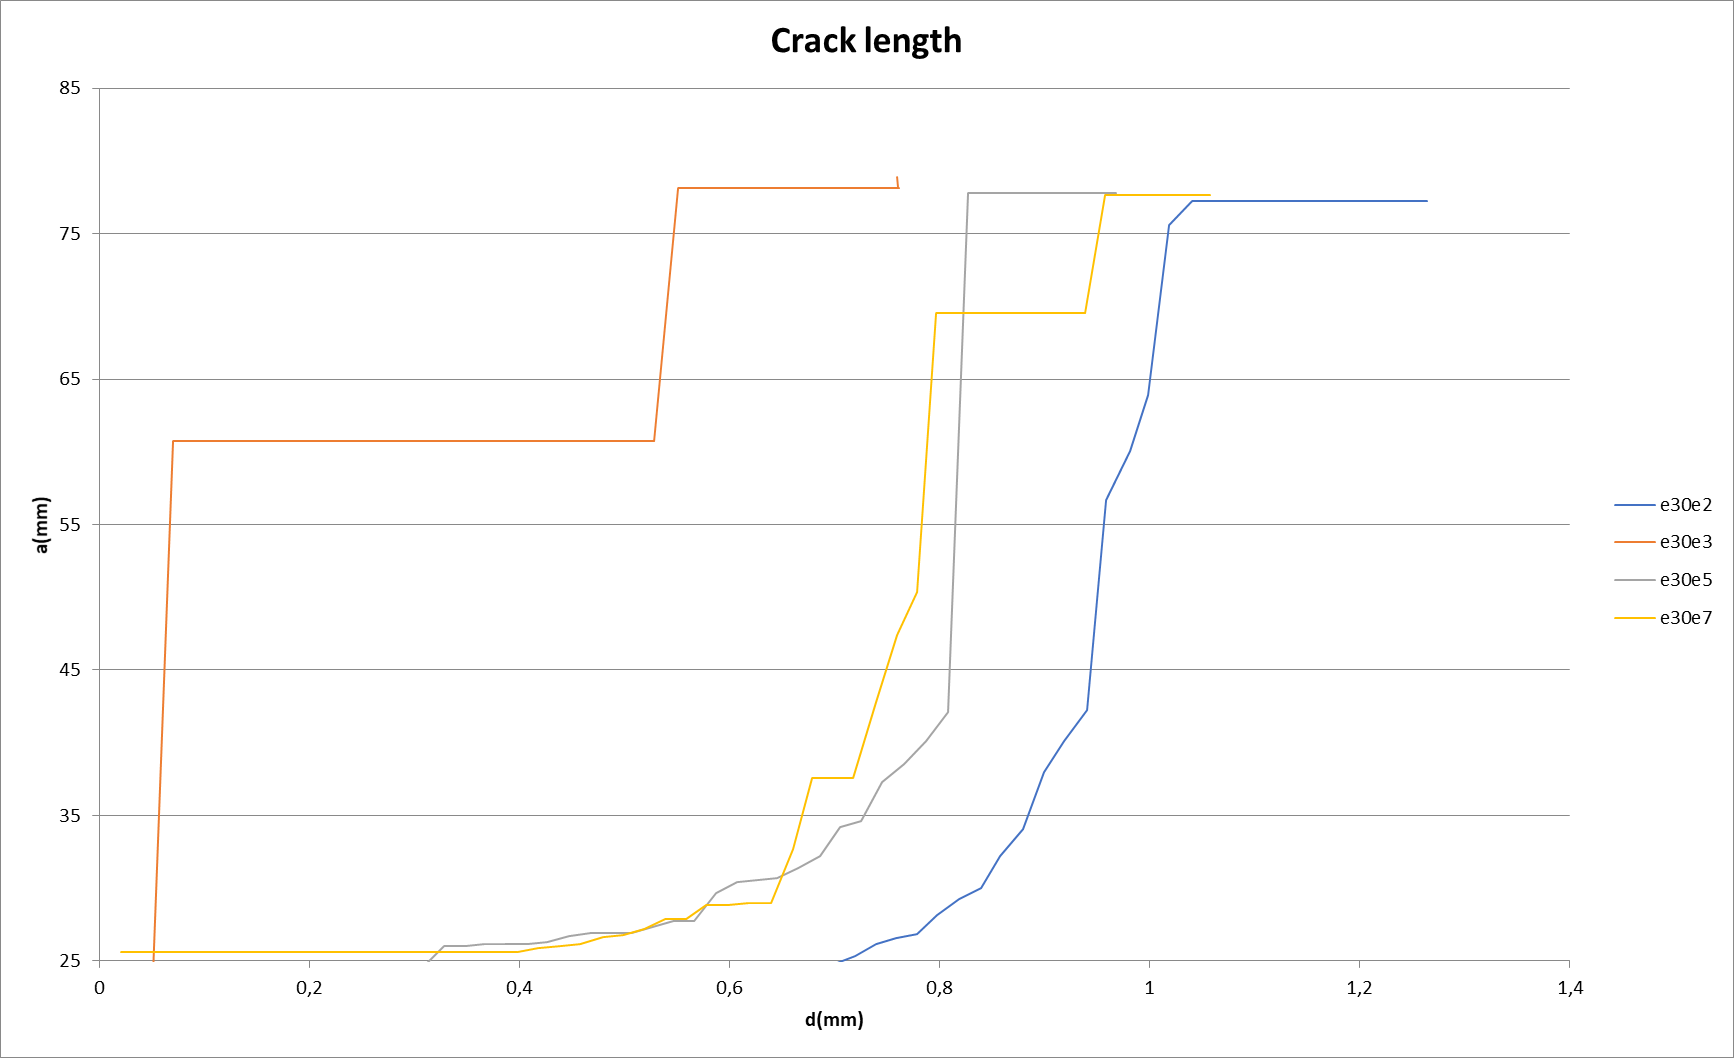
\includegraphics[width=13cm]{crack_30}
	\caption{Crack length evolution for 30°}
	\label{fig:crack_30}
\end{figure}

\subsection{Critical energy restitution rate}

Figures \ref{fig:G1_15} and \ref{fig:G2_15} below show the decoupled restitution rate for the mixed mode with 15°.
As for mode I, depending on the specimen, different values of a(t) are reached with the maximum energy restitution rate for the mode I and mode II part. For values of a(t) between 52 and 80 mm, the mode I part reaches $GI_{max}$, whereas for the mode II part for values of a(t) between 38 and 64mm, the mode II part reaches $GII_{max}$. This difference in a(t) for $GI_{max}$ and $GII_{max}$ can be explained by the CTOD measurements for mode I and mode II.
In addition, we can see that the curves of G reach a certain plateau which corresponds to the desired shape of the plot of the energy restitution rate. Indeed, the MMCG specimen has an increasing inertia with respect to the crack tip in order to guarantee the stability of the energy restitution rate.

\begin{figure}[htp]
	\centering
	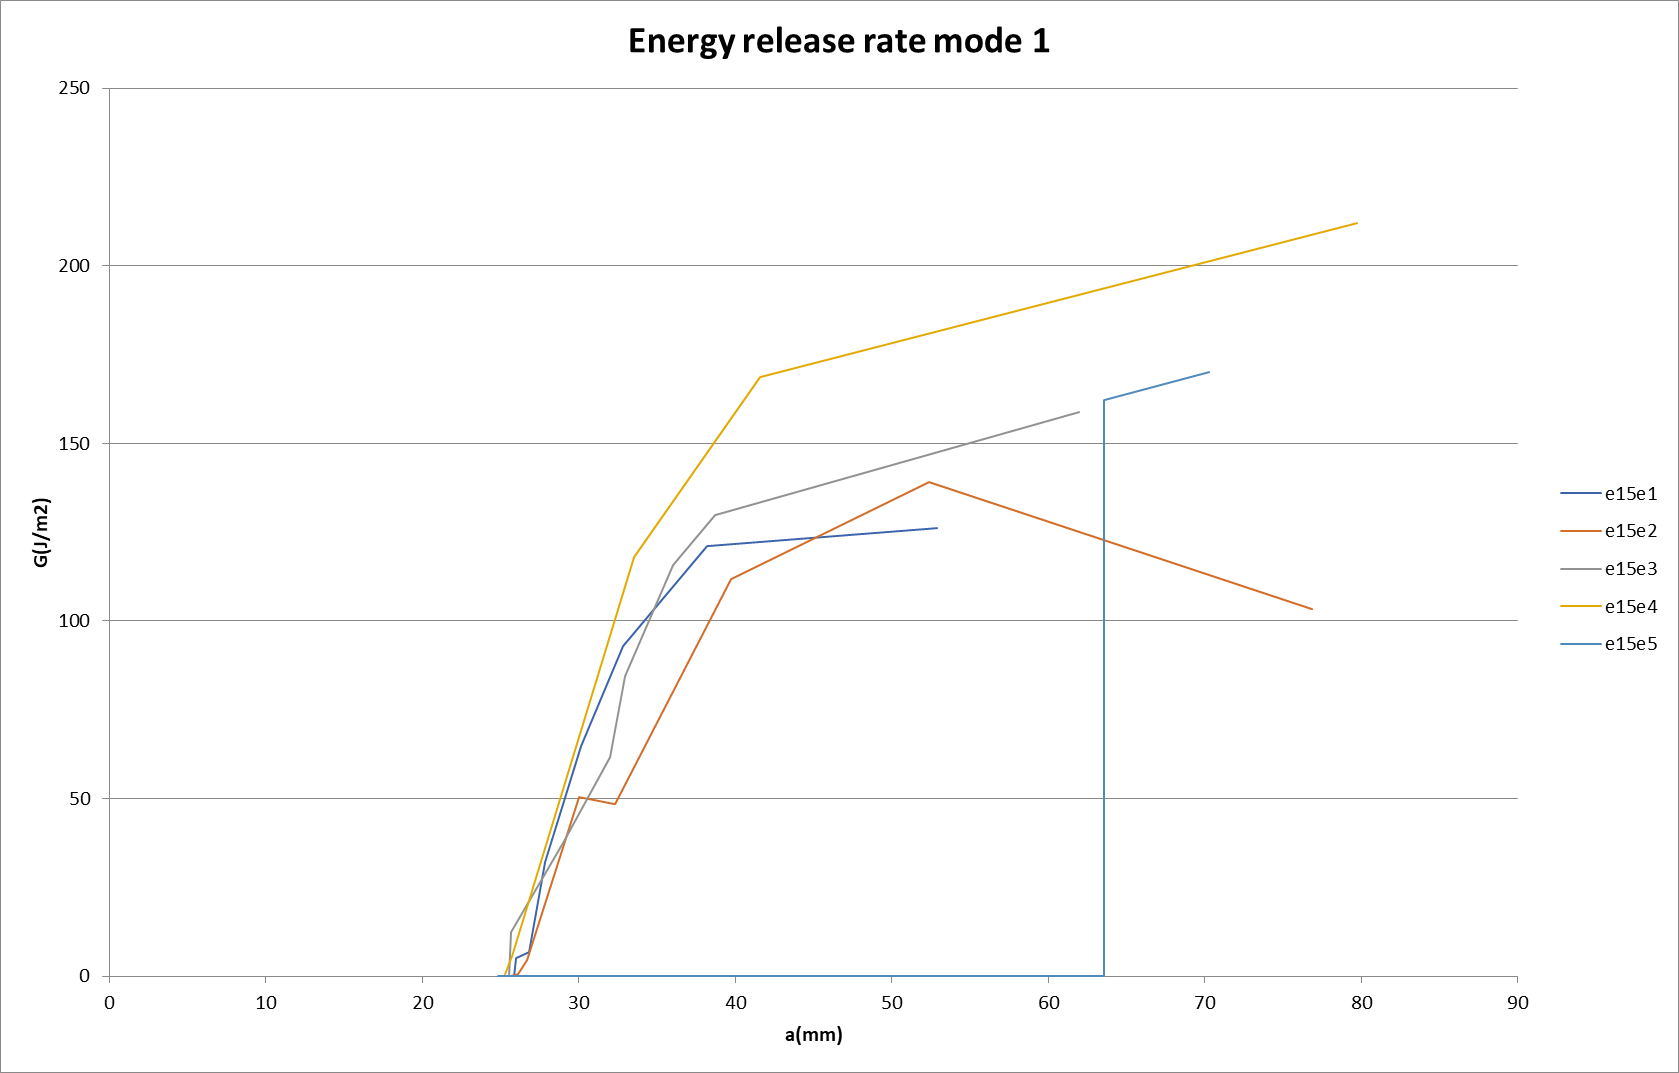
\includegraphics[width=12.5cm]{G1_15}
	\caption{Energy restitution rate as a function of crack length for 15°; mode I share}
	\label{fig:G1_15}
\end{figure}

\begin{figure}[htp]
	\centering
	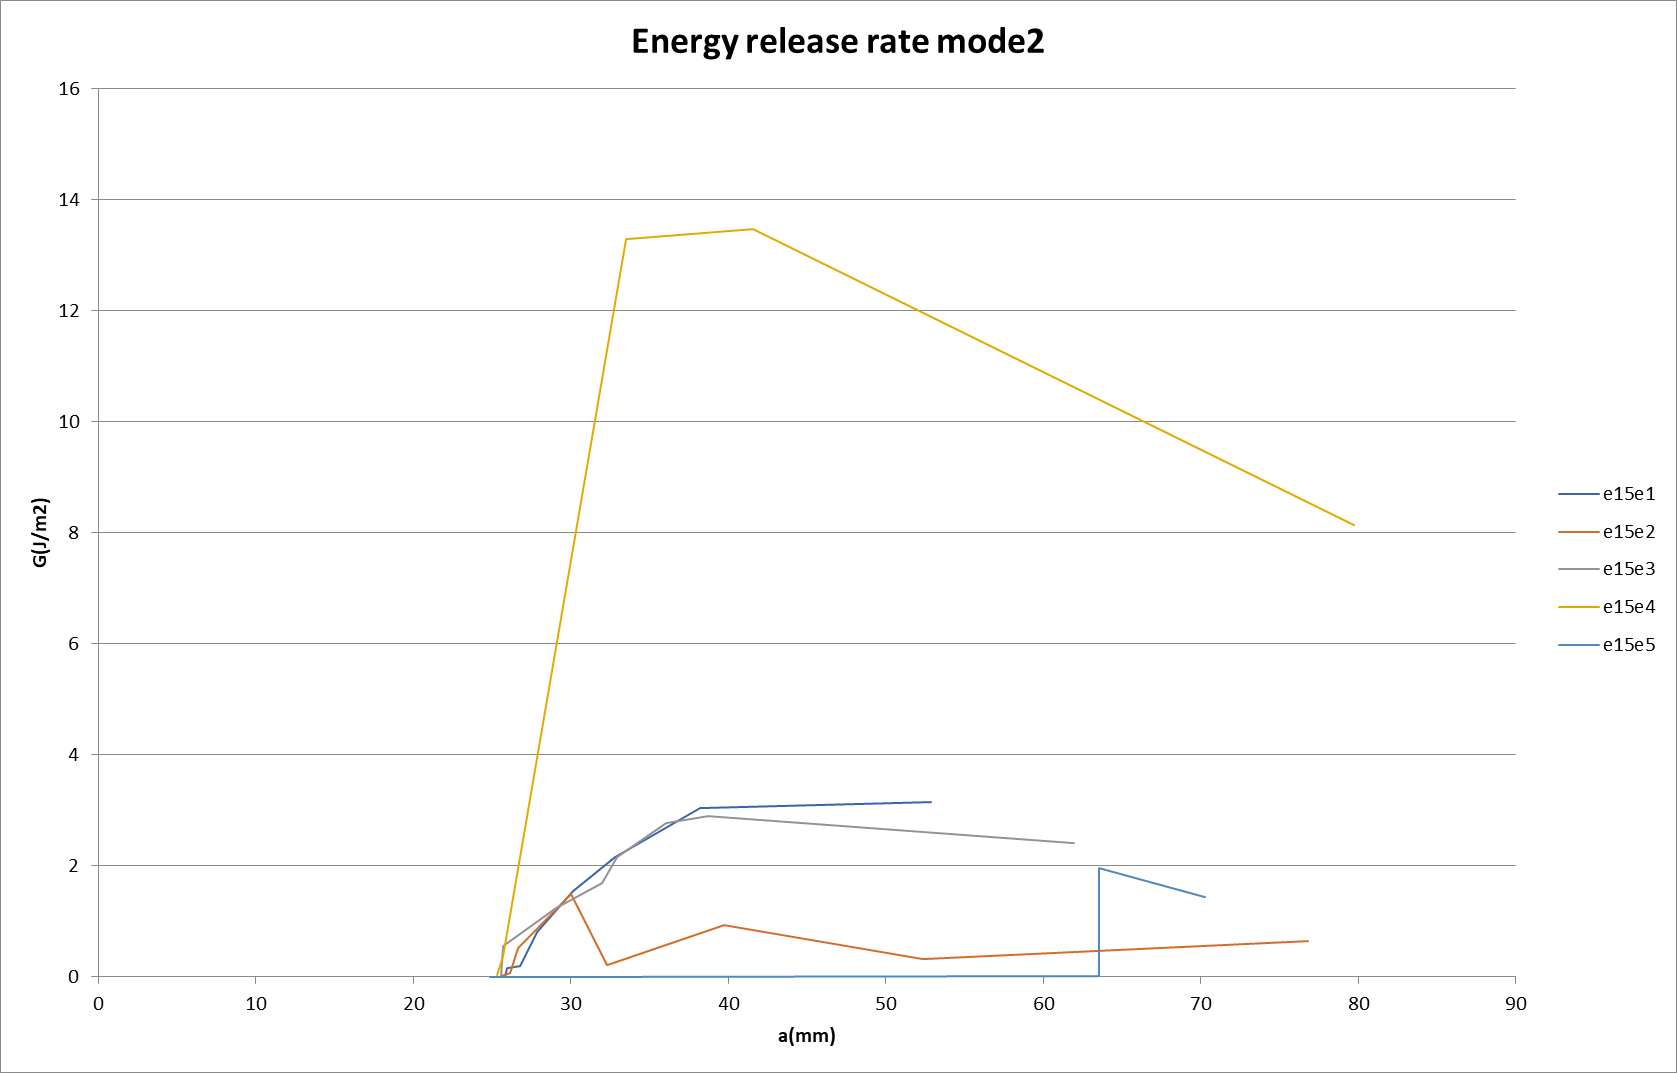
\includegraphics[width=12.5cm]{G2_15}
	\caption{Energy restitution rate as a function of crack length for 15°; mode II share}
	\label{fig:G2_15}
\end{figure}

Table \ref{fig:tableG15} gives the maximum values of GI and GII for 15°. There is a clear predominance of mode I over mode 2. In addition, the standard deviation is fairly low for mode I and seems relatively higher for mode 2 due to the value of G2 obtained by e15e4.

\begin{table} [H]
	\centering
	\begin{tabular}{ccccccccc}
		\toprule % horizontal line at the top of the table
		&  & e15e1 & e15e2 & e15e3 & e15e4 & e15e5 & Mean & Standard deviation\\\midrule
		& $GI_{max}, (J/m^2)$ & 126.21 & 139.19 & 158.93 & 212.07 & 169.98 & 161.28 & 33.09 \\\midrule
		& $GII_{max}, (J/m^2)$ & 3.15 & 0.93 & 2.90 & 13.48 & 1.95 & 4.60 & 5.01\\\midrule
	\end{tabular}
	\caption{$G_{max}$ values for Silver Fir specimens in mixed mode for 15°}
	\label{fig:tableG15}
\end{table}

Figures \ref{fig:G1_30} and \ref{fig:G2_30} below show the decoupled restitution rate for the mixed mode with 30°.
We can see that for values of a(t) between 42 and 78 mm, the mode I part reaches $GI_{max}$, whereas for the mode 2 part, for values of a(t) between 32 and 61 mm, the mode 2 part reaches G2max. 

\begin{figure}[htp]
	\centering
	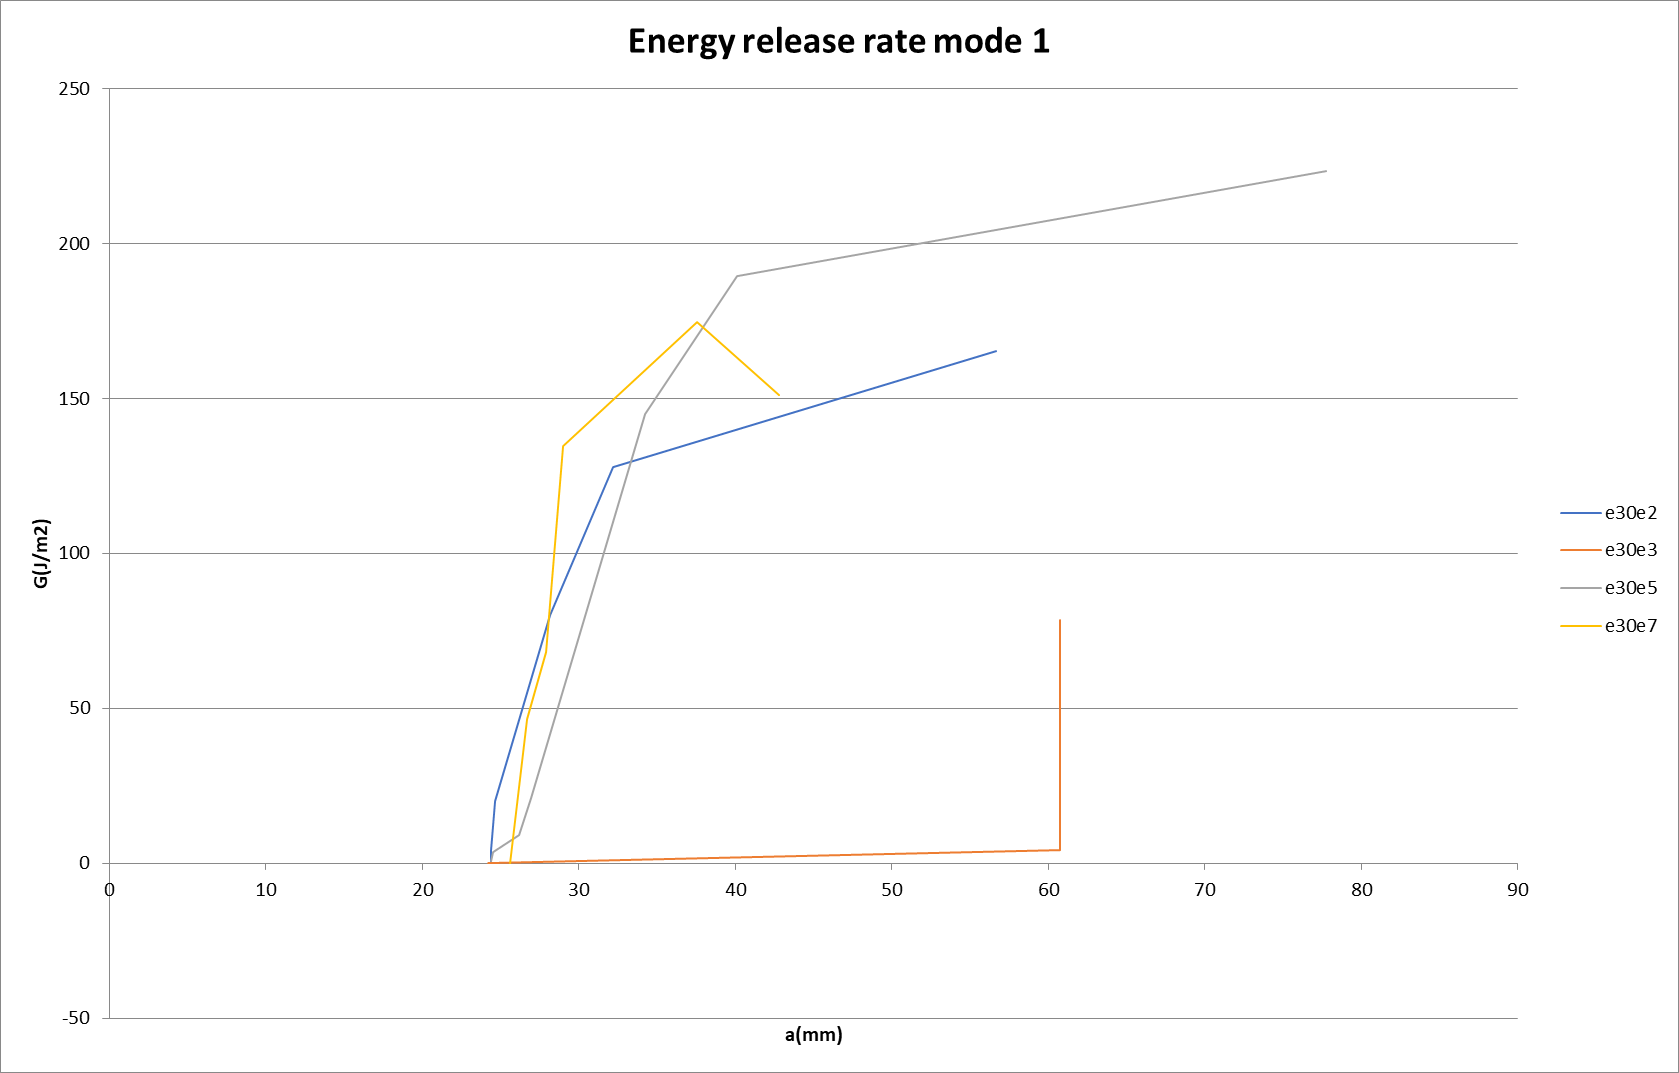
\includegraphics[width=12.5cm]{G1_30}
	\caption{Energy restitution rate as a function of crack length for 30°; mode I share}
	\label{fig:G1_30}
\end{figure}


\begin{figure}[htp]
	\centering
	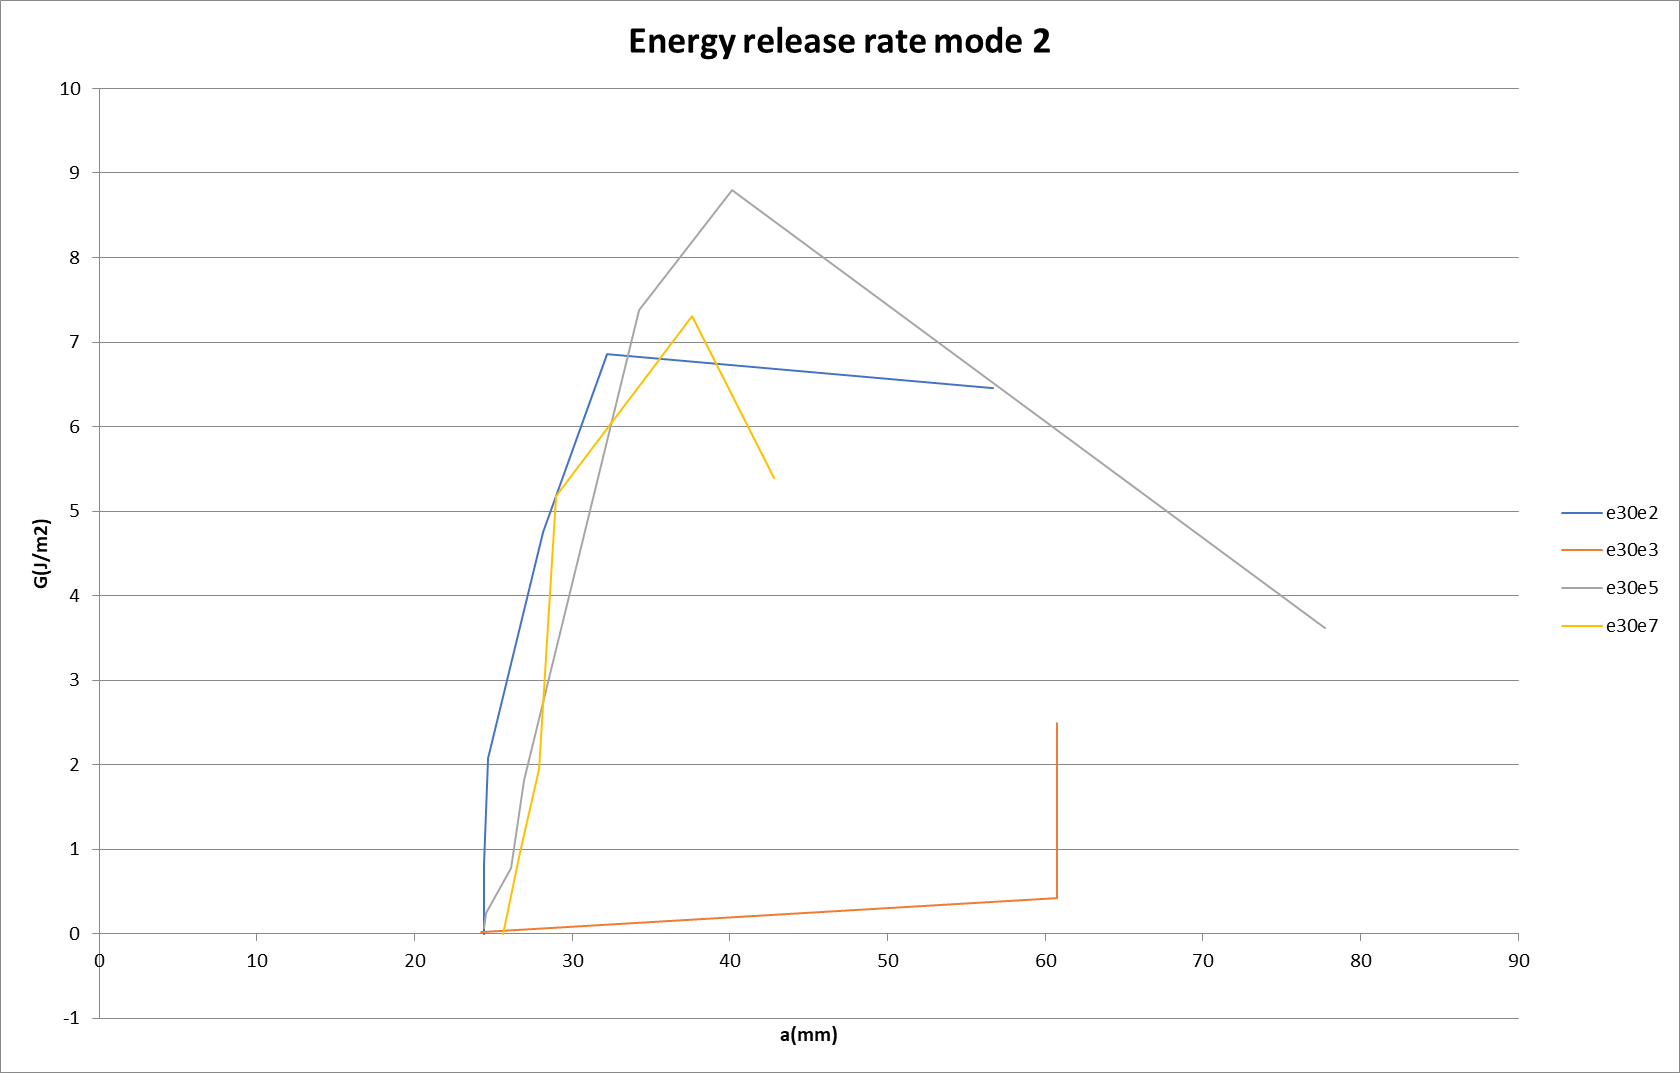
\includegraphics[width=12.5cm]{G2_30}
	\caption{Energy restitution rate as a function of crack length for 30°; mode II share}
	\label{fig:G2_30}
\end{figure}

Table \ref{fig:tableG30} gives the maximum values of GI and GII for 30°. The values are similar to those for 15°, but there is a slight increase in G2.

\begin{table} [H]
	\centering
	\begin{tabular}{cccccccc}
		\toprule % horizontal line at the top of the table
		&  & e30e2 & e30e3 & e30e5 & e30e7 & Mean & Standard deviation\\\midrule
		& $GI_{max}, (J/m^2)$ & 165.38 & 78.58 & 223.31 & 174.74 & 160.50 & 60.23 \\\midrule
		& $GII_{max}, (J/m^2)$ & 6.86 & 2.49 & 8.80 & 7.31 & 6.37 & 2.71\\\midrule
	\end{tabular}
	\caption{$G_{max}$ values for Silver Fir specimens in mixed mode for 30°}
	\label{fig:tableG30}
\end{table}

\section{Discussion of the results}

\subsection{Data analysis and comparison}

Table \ref{fig:Comparison_angle} shows the average Gmax values for the different mixing angles.  It also shows the breaking force applied to the specimen for the 3 angles. The differences between modes I and II are compared.

\begin{table} [H]
	\centering
	\begin{tabular}{ccccccccc}
		\toprule % horizontal line at the top of the table
		&  & 0° & 15° & 30° \\\midrule
		& $GI_{max}, (J/m^2)$ & 170 & 161.28 & 160.5  \\\midrule
		& $GII_{max}, (J/m^2)$ & 0 & 4.6 & 6.37 \\\midrule
		& $GII_{max}$ -$GI_{max}, (J/m^2)$ & 170 & 156.68 & 154.13 \\\midrule
		& $P_{max}$, (N) & 395.8 & 433.8 & 457.3 \\\midrule
	\end{tabular}
	\caption{Comparison of the energy restitution rate as a function of the mixing angle}
	\label{fig:Comparison_angle}
\end{table}

Depending on the different mixing angles, we can see a slight decrease in the difference between mode I and mode II as the mixing angle increases.

After analysis of the tests for the different mix ratios, the results obtained gave the following information:

For all the mix angles studied, the mode I share is always higher than the mode II share.

The breaking force provided to the specimen increases with the increase of the mixing angle. This can be explained by the fact that the resistance is maximum for a load parallel to the fibres.

The energy restitution rate values from mode I decrease with increasing degree of mixing angle, while the energy restitution rate values from mode II increase, as is the case for \cite{Odounga2018phd}. However, in this case, this variation is very small, and tests should have been carried out with a larger mixing angle to verify better this hypothesis.

The difference between GI and GII decreases with increasing mixing angle, which at the same time justifies the complete decoupling of mixed failure modes. There is a decreasing trend in the GI-GII difference. 
In the results obtained by \cite{Odounga2018phd}, it is when approaching an angle of 45 degrees that the crack opening values along x and y tend to approach each other. In mixed mode, the crack opening is no longer one-dimensional since the specimen is stressed at an angle that induces the cohabitation of two modes, which leads to a projection along both axes of the crack opening. Obtaining the two components u and v leads to the calculation of GI and GII . In other words, the two modes are decoupled. The difference between the values of the two modes is therefore greatest when the mixing angle is as small as possible. According to \cite{Odounga2018phd} , this difference decreases up to an angle of 45 degrees, where it is minimal. Between 0 and 45 degrees, mode I is greater than mode II. It is probably after a mixing angle of 45 degrees that mode II is expected to be superior to mode 1.

Moreover, the results seem consistent with those obtained by \cite{MoutouPitti2008} with douglas fir specimens. For a mixing angle of 15 degrees, he obtained $GI_{max}$=250 J/m2 and $GII_{max}$=8J/m2 experimentally. For 30°, he obtained $GI_{max}$=270J/m2 and $GII_{max}$=18J/m2, which are broadly the same results obtained in this report.
However, the values obtained by \cite{Odounga2018phd} in mixed mode are different, since he obtains values for GI of the order of $10^2 J/m^2$.

\subsection{Difficulties and improvements}

Other researchers can continue the study, and numerous improvements can be made. The specimens' preparation, content, and shape all need to be carefully controlled. Indeed, even while the thickness, precrack, and other characteristics that we measured are taken into consideration in the calculations and tests, these are still approximations. Therefore, having very slight bias in all of these parameters has an impact on the final results.

One problem with this work was also the raw data from the servo-hydraulic press device. Indeed, as explained, an offset was applied to the P-delta curve to avoid negative values that made no sense. It was decided to shift P with its minimal value to account for the preload. In some situations, the last index of P was lower than the first index and that the machine appears to be able to move freely for the last indices of P without any change in the force P. Therefore, we decided that this delta P matched the preload. However, in some cases, the machine cannot be seen to move freely without a change in the force P for the last indices of P. As a result, the preload is sometimes underestimated because there is some preload tension that cannot be measured.
By roughly estimating this first load, all the results are slightly truncated and there is an impact on the other parameters. Incorrect values have an impact on these calculations since the load P is required to determine Compliance and the energy release rate. The square factor applied to the load parameter has a special impact on G. Before using the hydraulic press, it is essential to check the load in order to solve this issue. 

Another problem is illustrated by figure \ref{fig:Crack_junction}. The MMCG specimen has a crack at the connection fillet. Indeed, among the difficulties encountered, the brittleness of the specimens at the level of the connection fillet is precisely the one that caused the most problems. It is for this reason that several tests were not used. Three tests with a 30° angle and one test with a 45° angle broke at the connection fillet. One specimen at 0° did not crack at the initial crack tip and finally one specimen broke because the machine stopped abruptly during the test because it was overheating. In conclusion, fourteen tests were successful and it was only possible to analyse for the 0°, 15° and 30° angles. In future tests, it will be important to reinforce the specimen in some areas.

\begin{figure}[htp]
	\centering
	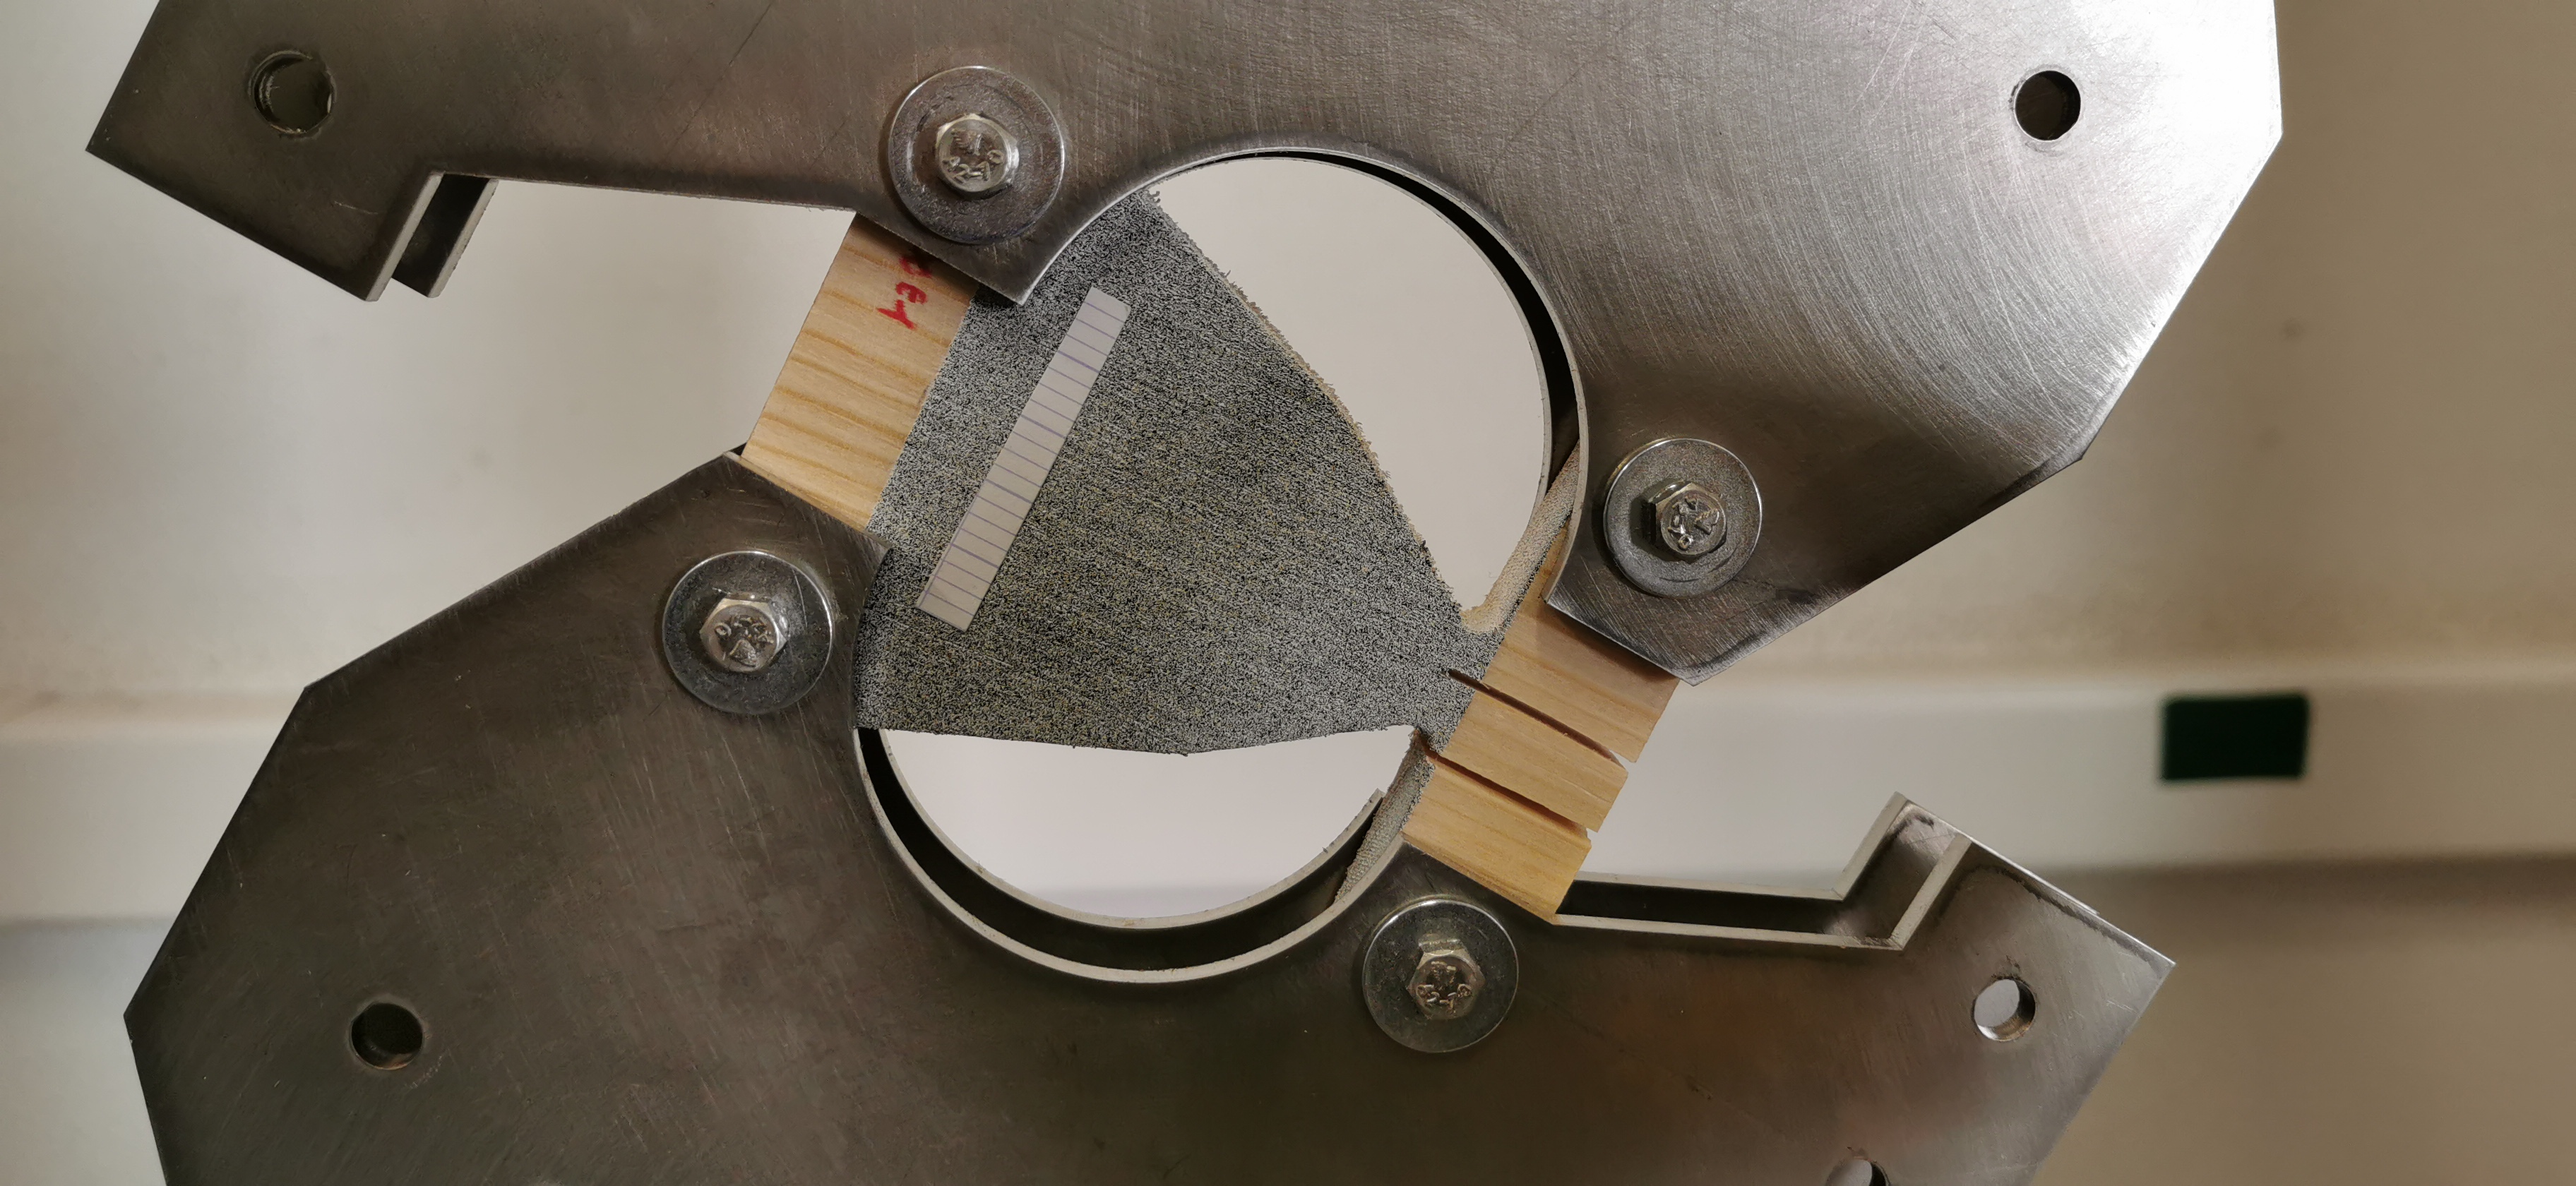
\includegraphics[width=12cm]{Crack_junction}
	\caption{Fracture issues encountered at the connection fillets}
	\label{fig:Crack_junction}
\end{figure}

Various methods of calculating G were tested. It was considered to use compliance as a function derived from the crack length. In order to make a(t) smoother, we decided to take only the indices of a(t) when propagation occurs. In other words, we removed the duplicate a(t). We then tried to interpolate a(t) with different functions. However, the interpolated functions did not fit well at all points.
Finally, it was decided to use the same methodology as \cite{MoutouPitti2008}, \cite{Mambili2018} and  \cite{Odounga2018phd}, i.e. to take only the indices where there is a critical force signifying a crack propagation and calculating $\Delta c$/$\Delta a$ between the starting point and the point considered for all the critical forces.

In this study, it was not possible to compare the results obtained with the Abaqus software. This comparison could provide a better understanding of the behaviour of wood and enable the results to be verified. A colleague at the university who is also doing a thesis master's degree is currently working on the finite element method to compare the results obtained in this work with those he will obtain numerically. In addition, it might be interesting to carry out more tests with softwood specimens in mode I and mixed mode, since only fourteen specimens were tested in this study.
Finally, it might be worth considering a solution to prevent the specimens from breaking at the fillet connection.

\section{Conclusion}

In this chapter, MMCG specimens were used to study the mixed-mode cracking of Silver Fir. A tensile testing machine was used to perform the tensile tests for the 15° and 30° mixed angles. Tests at an angle of 45° degrees could not be carried out because too many specimens broke at the fillet connection. The decoupling of modes gave the share of modes I and II.  Typical deformation maps and results in terms of force as a function of crack opening and energy restitution rate as a function of crack length were presented. The various results of the energy restitution rates calculated by the compliance method at imposed displacement showed a predominance of mode 1 over mode 2, with a reduction in this predominance as the mixing angle is increased.